\documentclass[tikz,border=12pt]{standalone}
\usepackage[T1]{fontenc}
\usetikzlibrary{calc}
\begin{document}
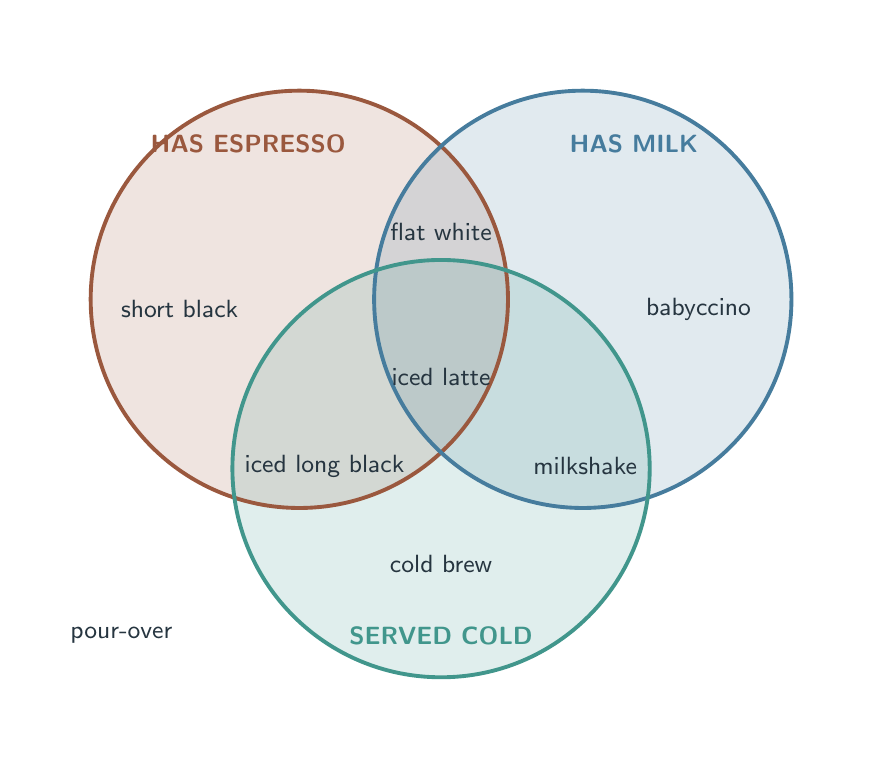
\begin{tikzpicture}[font=\sffamily]
  \definecolor{espresso}{HTML}{9A583E}
  \definecolor{milk}{HTML}{467C9D}
  \definecolor{cold}{HTML}{41968C}
  \definecolor{ink}{HTML}{263540}
  \path[use as bounding box] (-5.25,-4.7) rectangle (5.25,4.25);

  % Transparent washes show every intersection without hiding its neighbours.
  \fill[espresso,opacity=.16] (-1.8,.8) circle (2.65);
  \fill[milk,opacity=.16] (1.8,.8) circle (2.65);
  \fill[cold,opacity=.16] (0,-1.35) circle (2.65);
  \draw[espresso,line width=1.4pt] (-1.8,.8) circle (2.65);
  \draw[milk,line width=1.4pt] (1.8,.8) circle (2.65);
  \draw[cold,line width=1.4pt] (0,-1.35) circle (2.65);

  \tikzset{heading/.style={font=\sffamily\bfseries\small,inner sep=1pt},
           drink/.style={font=\sffamily\small,text=ink,align=center,inner sep=1pt}}
  \node[heading,text=espresso] at (-2.45,2.78) {HAS ESPRESSO};
  \node[heading,text=milk] at (2.45,2.78) {HAS MILK};
  \node[heading,text=cold] at (0,-3.48) {SERVED COLD};

  \node[drink] at (-3.32,.68) {short black};
  \node[drink] at (3.27,.68) {babyccino};
  \node[drink] at (0,1.66) {flat white};
  \node[drink] at (-1.48,-1.32) {iced long black};
  \node[drink] at (1.83,-1.32) {milkshake};
  \node[drink] at (0,-.19) {iced latte};
  \node[drink] at (0,-2.56) {cold brew};
  \node[drink] at (-4.06,-3.47) {pour-over};
\end{tikzpicture}
\end{document}
